\documentclass{standalone}
\usepackage{tikz}
\usetikzlibrary{patterns, positioning}

\begin{document}
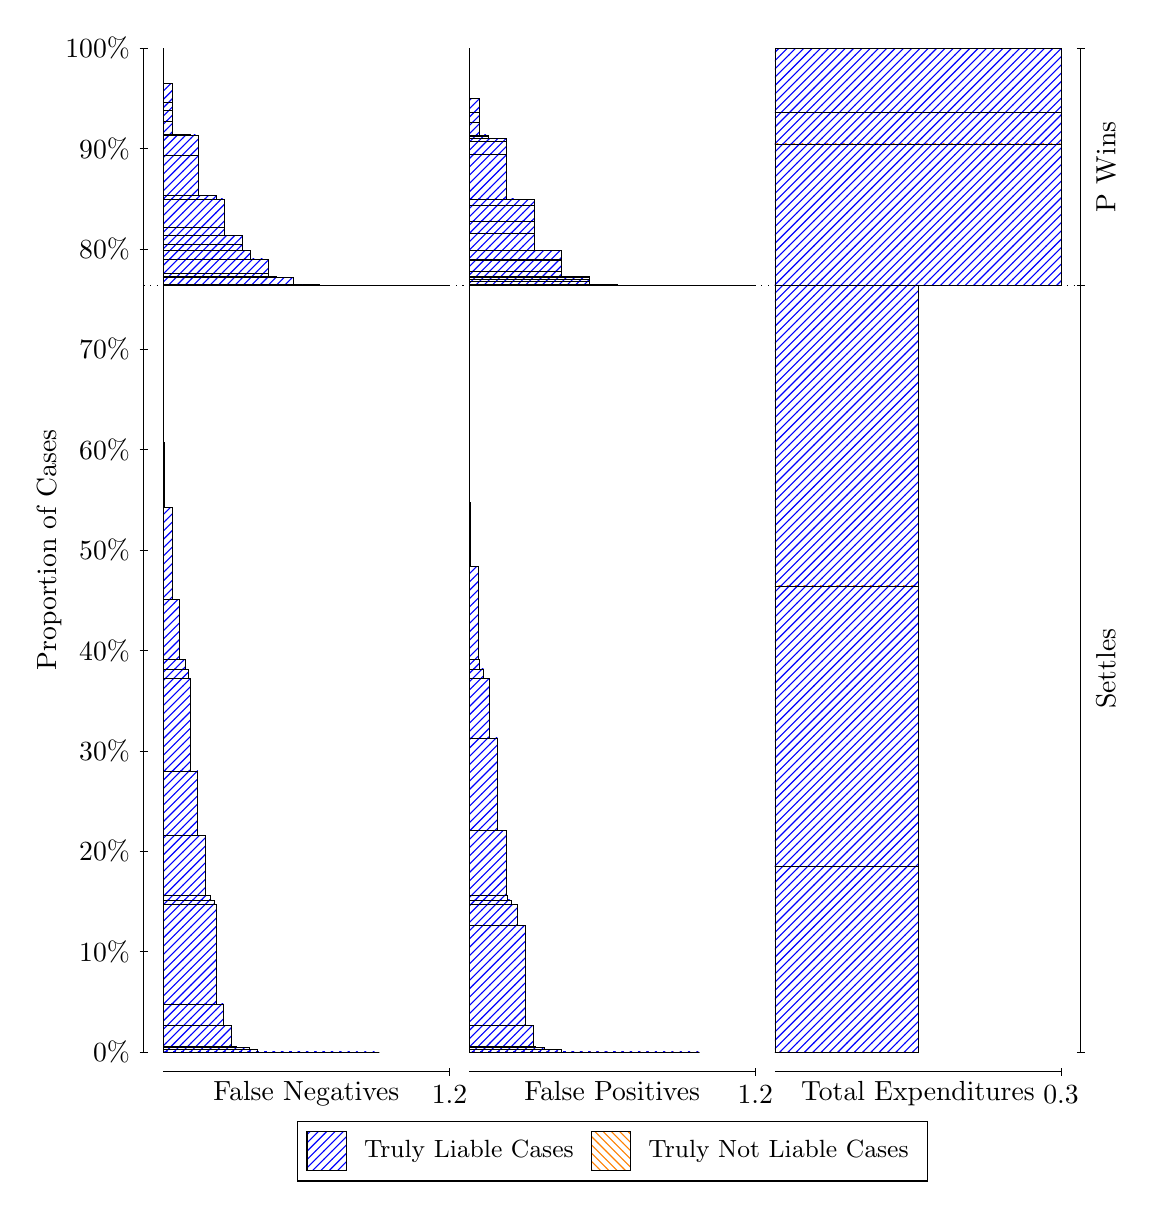
\begin{tikzpicture}
\draw[black, very thin] (1.5,1.75) -- (1.5,14.5);
\node[rotate=90, anchor=center] at (0.3, 8.125) {Proportion of Cases};
\draw[black, very thin] (1.45,1.75) -- (1.55,1.75);
\node[anchor=east] at (1.45, 1.75) {0\%};
\draw[black, very thin] (1.45,3.025) -- (1.55,3.025);
\node[anchor=east] at (1.45, 3.025) {10\%};
\draw[black, very thin] (1.45,4.3) -- (1.55,4.3);
\node[anchor=east] at (1.45, 4.3) {20\%};
\draw[black, very thin] (1.45,5.575) -- (1.55,5.575);
\node[anchor=east] at (1.45, 5.575) {30\%};
\draw[black, very thin] (1.45,6.85) -- (1.55,6.85);
\node[anchor=east] at (1.45, 6.85) {40\%};
\draw[black, very thin] (1.45,8.125) -- (1.55,8.125);
\node[anchor=east] at (1.45, 8.125) {50\%};
\draw[black, very thin] (1.45,9.4) -- (1.55,9.4);
\node[anchor=east] at (1.45, 9.4) {60\%};
\draw[black, very thin] (1.45,10.675) -- (1.55,10.675);
\node[anchor=east] at (1.45, 10.675) {70\%};
\draw[black, very thin] (1.45,11.95) -- (1.55,11.95);
\node[anchor=east] at (1.45, 11.95) {80\%};
\draw[black, very thin] (1.45,13.225) -- (1.55,13.225);
\node[anchor=east] at (1.45, 13.225) {90\%};
\draw[black, very thin] (1.45,14.5) -- (1.55,14.5);
\node[anchor=east] at (1.45, 14.5) {100\%};

\draw[black, very thin] (13.4,1.75) -- (13.4,14.5);
\draw[black, very thin] (13.35,1.75) -- (13.45,1.75);
\node[anchor=west] at (13.35, 1.75) {};
\draw[black, very thin] (13.35,11.482) -- (13.45,11.482);
\node[anchor=west] at (13.35, 11.482) {};
\draw[black, very thin] (13.35,14.5) -- (13.45,14.5);
\node[anchor=west] at (13.35, 14.5) {};

\draw[black, very thin, pattern color=blue, pattern=north east lines] (1.75,1.75) rectangle (4.4935,1.75);
\draw[black, very thin, pattern color=blue, pattern=north east lines] (1.75,1.75) rectangle (4.164,1.75);
\draw[black, very thin, pattern color=blue, pattern=north east lines] (1.75,1.75) rectangle (4.0486,1.75);
\draw[black, very thin, pattern color=blue, pattern=north east lines] (1.75,1.75) rectangle (3.8344,1.75);
\draw[black, very thin, pattern color=blue, pattern=north east lines] (1.75,1.75) rectangle (3.7191,1.75);
\draw[black, very thin, pattern color=blue, pattern=north east lines] (1.75,1.75) rectangle (3.6037,1.75);
\draw[black, very thin, pattern color=blue, pattern=north east lines] (1.75,1.75) rectangle (3.5049,1.75);
\draw[black, very thin, pattern color=blue, pattern=north east lines] (1.75,1.75) rectangle (3.4554,1.75);
\draw[black, very thin, pattern color=blue, pattern=north east lines] (1.75,1.75) rectangle (3.3895,1.75);
\draw[black, very thin, pattern color=blue, pattern=north east lines] (1.75,1.75) rectangle (3.2742,1.7506);
\draw[black, very thin, pattern color=blue, pattern=north east lines] (1.75,1.7506) rectangle (3.1753,1.7511);
\draw[black, very thin, pattern color=blue, pattern=north east lines] (1.75,1.7511) rectangle (3.1259,1.7511);
\draw[black, very thin, pattern color=blue, pattern=north east lines] (1.75,1.7511) rectangle (3.06,1.7513);
\draw[black, very thin, pattern color=blue, pattern=north east lines] (1.75,1.7513) rectangle (3.0105,1.7518);
\draw[black, very thin, pattern color=blue, pattern=north east lines] (1.75,1.7518) rectangle (2.9446,1.7784);
\draw[black, very thin, pattern color=blue, pattern=north east lines] (1.75,1.7784) rectangle (2.8458,1.8046);
\draw[black, very thin, pattern color=blue, pattern=north east lines] (1.75,1.8046) rectangle (2.7963,1.8046);
\draw[black, very thin, pattern color=blue, pattern=north east lines] (1.75,1.8046) rectangle (2.7304,1.8115);
\draw[black, very thin, pattern color=blue, pattern=north east lines] (1.75,1.8115) rectangle (2.681,1.8194);
\draw[black, very thin, pattern color=blue, pattern=north east lines] (1.75,1.8194) rectangle (2.6151,2.0889);
\draw[black, very thin, pattern color=blue, pattern=north east lines] (1.75,2.0889) rectangle (2.5162,2.3607);
\draw[black, very thin, pattern color=blue, pattern=north east lines] (1.75,2.3607) rectangle (2.4668,2.3608);
\draw[black, very thin, pattern color=blue, pattern=north east lines] (1.75,2.3608) rectangle (2.4173,3.6239);
\draw[black, very thin, pattern color=blue, pattern=north east lines] (1.75,3.6239) rectangle (2.4009,3.6823);
\draw[black, very thin, pattern color=blue, pattern=north east lines] (1.75,3.6823) rectangle (2.3514,3.7414);
\draw[black, very thin, pattern color=blue, pattern=north east lines] (1.75,3.7414) rectangle (2.2855,4.4983);
\draw[black, very thin, pattern color=blue, pattern=north east lines] (1.75,4.4983) rectangle (2.1867,5.3184);
\draw[black, very thin, pattern color=blue, pattern=north east lines] (1.75,5.3184) rectangle (2.1372,5.3189);
\draw[black, very thin, pattern color=blue, pattern=north east lines] (1.75,5.3189) rectangle (2.0878,6.4948);
\draw[black, very thin, pattern color=blue, pattern=north east lines] (1.75,6.4948) rectangle (2.0713,6.6161);
\draw[black, very thin, pattern color=blue, pattern=north east lines] (1.75,6.6161) rectangle (2.0219,6.7373);
\draw[black, very thin, pattern color=blue, pattern=north east lines] (1.75,6.7373) rectangle (1.956,7.4943);
\draw[black, very thin, pattern color=blue, pattern=north east lines] (1.75,7.4943) rectangle (1.8571,8.6701);
\draw[black, very thin, pattern color=blue, pattern=north east lines] (1.75,8.6701) rectangle (1.8077,8.6706);
\draw[black, very thin, pattern color=blue, pattern=north east lines] (1.75,8.6706) rectangle (1.7582,9.4907);
\draw[black, very thin, pattern color=orange, pattern=north west lines] (1.75,9.4907) rectangle (1.75,9.4907);
\draw[black, very thin, pattern color=blue, pattern=north east lines] (1.75,9.4907) rectangle (1.75,11.482);
\draw[black, very thin, pattern color=blue, pattern=north east lines] (1.75,11.482) rectangle (5.3833,11.482);
\draw[black, very thin, pattern color=blue, pattern=north east lines] (1.75,11.482) rectangle (5.0538,11.482);
\draw[black, very thin, pattern color=blue, pattern=north east lines] (1.75,11.482) rectangle (4.7242,11.482);
\draw[black, very thin, pattern color=blue, pattern=north east lines] (1.75,11.482) rectangle (4.5018,11.482);
\draw[black, very thin, pattern color=blue, pattern=north east lines] (1.75,11.482) rectangle (4.3947,11.482);
\draw[black, very thin, pattern color=blue, pattern=north east lines] (1.75,11.482) rectangle (4.1722,11.482);
\draw[black, very thin, pattern color=blue, pattern=north east lines] (1.75,11.482) rectangle (4.0651,11.483);
\draw[black, very thin, pattern color=blue, pattern=north east lines] (1.75,11.483) rectangle (4.0651,11.484);
\draw[black, very thin, pattern color=blue, pattern=north east lines] (1.75,11.484) rectangle (3.8427,11.484);
\draw[black, very thin, pattern color=blue, pattern=north east lines] (1.75,11.484) rectangle (3.8427,11.484);
\draw[black, very thin, pattern color=blue, pattern=north east lines] (1.75,11.484) rectangle (3.7356,11.491);
\draw[black, very thin, pattern color=blue, pattern=north east lines] (1.75,11.491) rectangle (3.7356,11.501);
\draw[black, very thin, pattern color=blue, pattern=north east lines] (1.75,11.501) rectangle (3.5131,11.501);
\draw[black, very thin, pattern color=blue, pattern=north east lines] (1.75,11.501) rectangle (3.406,11.591);
\draw[black, very thin, pattern color=blue, pattern=north east lines] (1.75,11.591) rectangle (3.1836,11.595);
\draw[black, very thin, pattern color=blue, pattern=north east lines] (1.75,11.595) rectangle (3.1836,11.6);
\draw[black, very thin, pattern color=blue, pattern=north east lines] (1.75,11.6) rectangle (3.0765,11.638);
\draw[black, very thin, pattern color=blue, pattern=north east lines] (1.75,11.638) rectangle (3.0765,11.823);
\draw[black, very thin, pattern color=blue, pattern=north east lines] (1.75,11.823) rectangle (2.854,11.931);
\draw[black, very thin, pattern color=blue, pattern=north east lines] (1.75,11.931) rectangle (2.7469,12.003);
\draw[black, very thin, pattern color=blue, pattern=north east lines] (1.75,12.003) rectangle (2.7469,12.12);
\draw[black, very thin, pattern color=blue, pattern=north east lines] (1.75,12.12) rectangle (2.5245,12.224);
\draw[black, very thin, pattern color=blue, pattern=north east lines] (1.75,12.224) rectangle (2.5245,12.584);
\draw[black, very thin, pattern color=blue, pattern=north east lines] (1.75,12.584) rectangle (2.4173,12.633);
\draw[black, very thin, pattern color=blue, pattern=north east lines] (1.75,12.633) rectangle (2.1949,13.136);
\draw[black, very thin, pattern color=blue, pattern=north east lines] (1.75,13.136) rectangle (2.1949,13.398);
\draw[black, very thin, pattern color=blue, pattern=north east lines] (1.75,13.398) rectangle (2.0878,13.402);
\draw[black, very thin, pattern color=blue, pattern=north east lines] (1.75,13.402) rectangle (1.8653,13.574);
\draw[black, very thin, pattern color=blue, pattern=north east lines] (1.75,13.574) rectangle (1.8653,13.704);
\draw[black, very thin, pattern color=blue, pattern=north east lines] (1.75,13.704) rectangle (1.8653,13.808);
\draw[black, very thin, pattern color=blue, pattern=north east lines] (1.75,13.808) rectangle (1.8653,14.051);
\draw[black, very thin, pattern color=blue, pattern=north east lines] (1.75,14.051) rectangle (1.7582,14.051);
\draw[black, very thin, pattern color=orange, pattern=north west lines] (1.75,14.051) rectangle (1.75,14.051);
\draw[black, very thin, pattern color=blue, pattern=north east lines] (1.75,14.051) rectangle (1.75,14.5);
\draw[black, very thin, pattern color=orange, pattern=north west lines] (5.6333,1.75) rectangle (8.5558,1.75);
\draw[black, very thin, pattern color=blue, pattern=north east lines] (5.6333,1.75) rectangle (8.5558,1.75);
\draw[black, very thin, pattern color=blue, pattern=north east lines] (5.6333,1.75) rectangle (8.2048,1.75);
\draw[black, very thin, pattern color=orange, pattern=north west lines] (5.6333,1.75) rectangle (7.9239,1.75);
\draw[black, very thin, pattern color=blue, pattern=north east lines] (5.6333,1.75) rectangle (7.9239,1.75);
\draw[black, very thin, pattern color=blue, pattern=north east lines] (5.6333,1.75) rectangle (7.8537,1.75);
\draw[black, very thin, pattern color=blue, pattern=north east lines] (5.6333,1.75) rectangle (7.5729,1.75);
\draw[black, very thin, pattern color=blue, pattern=north east lines] (5.6333,1.75) rectangle (7.5027,1.75);
\draw[black, very thin, pattern color=orange, pattern=north west lines] (5.6333,1.75) rectangle (7.45,1.75);
\draw[black, very thin, pattern color=blue, pattern=north east lines] (5.6333,1.75) rectangle (7.45,1.75);
\draw[black, very thin, pattern color=orange, pattern=north west lines] (5.6333,1.75) rectangle (7.292,1.75);
\draw[black, very thin, pattern color=blue, pattern=north east lines] (5.6333,1.75) rectangle (7.292,1.75);
\draw[black, very thin, pattern color=blue, pattern=north east lines] (5.6333,1.75) rectangle (7.2218,1.75);
\draw[black, very thin, pattern color=blue, pattern=north east lines] (5.6333,1.75) rectangle (7.1516,1.7505);
\draw[black, very thin, pattern color=blue, pattern=north east lines] (5.6333,1.7505) rectangle (7.099,1.7505);
\draw[black, very thin, pattern color=blue, pattern=north east lines] (5.6333,1.7505) rectangle (6.941,1.7511);
\draw[black, very thin, pattern color=blue, pattern=north east lines] (5.6333,1.7511) rectangle (6.8708,1.7513);
\draw[black, very thin, pattern color=orange, pattern=north west lines] (5.6333,1.7513) rectangle (6.8181,1.7513);
\draw[black, very thin, pattern color=blue, pattern=north east lines] (5.6333,1.7513) rectangle (6.8181,1.7518);
\draw[black, very thin, pattern color=blue, pattern=north east lines] (5.6333,1.7518) rectangle (6.8006,1.7781);
\draw[black, very thin, pattern color=blue, pattern=north east lines] (5.6333,1.7781) rectangle (6.7479,1.7781);
\draw[black, very thin, pattern color=blue, pattern=north east lines] (5.6333,1.7781) rectangle (6.5899,1.8046);
\draw[black, very thin, pattern color=blue, pattern=north east lines] (5.6333,1.8046) rectangle (6.5197,1.8115);
\draw[black, very thin, pattern color=blue, pattern=north east lines] (5.6333,1.8115) rectangle (6.4671,1.8194);
\draw[black, very thin, pattern color=blue, pattern=north east lines] (5.6333,1.8194) rectangle (6.4495,2.0912);
\draw[black, very thin, pattern color=blue, pattern=north east lines] (5.6333,2.0912) rectangle (6.3969,2.0913);
\draw[black, very thin, pattern color=orange, pattern=north west lines] (5.6333,2.0913) rectangle (6.3442,2.0913);
\draw[black, very thin, pattern color=blue, pattern=north east lines] (5.6333,2.0913) rectangle (6.3442,3.3544);
\draw[black, very thin, pattern color=blue, pattern=north east lines] (5.6333,3.3544) rectangle (6.2389,3.6239);
\draw[black, very thin, pattern color=blue, pattern=north east lines] (5.6333,3.6239) rectangle (6.1687,3.6823);
\draw[black, very thin, pattern color=blue, pattern=north east lines] (5.6333,3.6823) rectangle (6.116,3.7414);
\draw[black, very thin, pattern color=blue, pattern=north east lines] (5.6333,3.7414) rectangle (6.0985,4.5614);
\draw[black, very thin, pattern color=blue, pattern=north east lines] (5.6333,4.5614) rectangle (6.0458,4.562);
\draw[black, very thin, pattern color=blue, pattern=north east lines] (5.6333,4.562) rectangle (5.9932,5.7378);
\draw[black, very thin, pattern color=blue, pattern=north east lines] (5.6333,5.7378) rectangle (5.8878,6.4948);
\draw[black, very thin, pattern color=blue, pattern=north east lines] (5.6333,6.4948) rectangle (5.8176,6.616);
\draw[black, very thin, pattern color=blue, pattern=north east lines] (5.6333,6.616) rectangle (5.765,6.7373);
\draw[black, very thin, pattern color=blue, pattern=north east lines] (5.6333,6.7373) rectangle (5.7474,7.9131);
\draw[black, very thin, pattern color=blue, pattern=north east lines] (5.6333,7.9131) rectangle (5.6948,7.9137);
\draw[black, very thin, pattern color=blue, pattern=north east lines] (5.6333,7.9137) rectangle (5.6421,8.7338);
\draw[black, very thin, pattern color=blue, pattern=north east lines] (5.6333,8.7338) rectangle (5.6333,11.482);
\draw[black, very thin, pattern color=orange, pattern=north west lines] (5.6333,11.482) rectangle (9.2667,11.482);
\draw[black, very thin, pattern color=blue, pattern=north east lines] (5.6333,11.482) rectangle (9.2667,11.482);
\draw[black, very thin, pattern color=orange, pattern=north west lines] (5.6333,11.482) rectangle (8.9156,11.482);
\draw[black, very thin, pattern color=blue, pattern=north east lines] (5.6333,11.482) rectangle (8.9156,11.482);
\draw[black, very thin, pattern color=orange, pattern=north west lines] (5.6333,11.482) rectangle (8.5646,11.482);
\draw[black, very thin, pattern color=blue, pattern=north east lines] (5.6333,11.482) rectangle (8.5646,11.482);
\draw[black, very thin, pattern color=blue, pattern=north east lines] (5.6333,11.482) rectangle (8.5646,11.482);
\draw[black, very thin, pattern color=blue, pattern=north east lines] (5.6333,11.482) rectangle (8.5646,11.482);
\draw[black, very thin, pattern color=orange, pattern=north west lines] (5.6333,11.482) rectangle (8.2135,11.482);
\draw[black, very thin, pattern color=blue, pattern=north east lines] (5.6333,11.482) rectangle (8.2135,11.482);
\draw[black, very thin, pattern color=blue, pattern=north east lines] (5.6333,11.482) rectangle (8.2135,11.482);
\draw[black, very thin, pattern color=orange, pattern=north west lines] (5.6333,11.482) rectangle (7.8625,11.482);
\draw[black, very thin, pattern color=blue, pattern=north east lines] (5.6333,11.482) rectangle (7.8625,11.483);
\draw[black, very thin, pattern color=blue, pattern=north east lines] (5.6333,11.483) rectangle (7.8625,11.484);
\draw[black, very thin, pattern color=blue, pattern=north east lines] (5.6333,11.484) rectangle (7.5114,11.49);
\draw[black, very thin, pattern color=orange, pattern=north west lines] (5.6333,11.49) rectangle (7.5114,11.49);
\draw[black, very thin, pattern color=blue, pattern=north east lines] (5.6333,11.49) rectangle (7.5114,11.494);
\draw[black, very thin, pattern color=blue, pattern=north east lines] (5.6333,11.494) rectangle (7.5114,11.501);
\draw[black, very thin, pattern color=orange, pattern=north west lines] (5.6333,11.501) rectangle (7.2745,11.501);
\draw[black, very thin, pattern color=blue, pattern=north east lines] (5.6333,11.501) rectangle (7.2745,11.501);
\draw[black, very thin, pattern color=blue, pattern=north east lines] (5.6333,11.501) rectangle (7.1604,11.532);
\draw[black, very thin, pattern color=blue, pattern=north east lines] (5.6333,11.532) rectangle (7.1604,11.559);
\draw[black, very thin, pattern color=orange, pattern=north west lines] (5.6333,11.559) rectangle (7.1604,11.559);
\draw[black, very thin, pattern color=blue, pattern=north east lines] (5.6333,11.559) rectangle (7.1604,11.584);
\draw[black, very thin, pattern color=blue, pattern=north east lines] (5.6333,11.584) rectangle (7.1604,11.6);
\draw[black, very thin, pattern color=orange, pattern=north west lines] (5.6333,11.6) rectangle (6.9234,11.6);
\draw[black, very thin, pattern color=blue, pattern=north east lines] (5.6333,11.6) rectangle (6.9234,11.6);
\draw[black, very thin, pattern color=blue, pattern=north east lines] (5.6333,11.6) rectangle (6.9234,11.6);
\draw[black, very thin, pattern color=blue, pattern=north east lines] (5.6333,11.6) rectangle (6.8093,11.668);
\draw[black, very thin, pattern color=orange, pattern=north west lines] (5.6333,11.668) rectangle (6.8093,11.668);
\draw[black, very thin, pattern color=blue, pattern=north east lines] (5.6333,11.668) rectangle (6.8093,11.808);
\draw[black, very thin, pattern color=blue, pattern=north east lines] (5.6333,11.808) rectangle (6.8093,11.82);
\draw[black, very thin, pattern color=blue, pattern=north east lines] (5.6333,11.82) rectangle (6.8093,11.931);
\draw[black, very thin, pattern color=orange, pattern=north west lines] (5.6333,11.931) rectangle (6.5724,11.931);
\draw[black, very thin, pattern color=blue, pattern=north east lines] (5.6333,11.931) rectangle (6.5724,11.931);
\draw[black, very thin, pattern color=blue, pattern=north east lines] (5.6333,11.931) rectangle (6.5724,11.931);
\draw[black, very thin, pattern color=blue, pattern=north east lines] (5.6333,11.931) rectangle (6.4583,12.151);
\draw[black, very thin, pattern color=blue, pattern=north east lines] (5.6333,12.151) rectangle (6.4583,12.304);
\draw[black, very thin, pattern color=blue, pattern=north east lines] (5.6333,12.304) rectangle (6.4583,12.498);
\draw[black, very thin, pattern color=blue, pattern=north east lines] (5.6333,12.498) rectangle (6.4583,12.58);
\draw[black, very thin, pattern color=orange, pattern=north west lines] (5.6333,12.58) rectangle (6.2213,12.58);
\draw[black, very thin, pattern color=blue, pattern=north east lines] (5.6333,12.58) rectangle (6.2213,12.584);
\draw[black, very thin, pattern color=blue, pattern=north east lines] (5.6333,12.584) rectangle (6.2213,12.584);
\draw[black, very thin, pattern color=blue, pattern=north east lines] (5.6333,12.584) rectangle (6.1072,13.155);
\draw[black, very thin, pattern color=blue, pattern=north east lines] (5.6333,13.155) rectangle (6.1072,13.316);
\draw[black, very thin, pattern color=blue, pattern=north east lines] (5.6333,13.316) rectangle (6.1072,13.349);
\draw[black, very thin, pattern color=blue, pattern=north east lines] (5.6333,13.349) rectangle (5.8703,13.378);
\draw[black, very thin, pattern color=orange, pattern=north west lines] (5.6333,13.378) rectangle (5.8703,13.378);
\draw[black, very thin, pattern color=blue, pattern=north east lines] (5.6333,13.378) rectangle (5.8703,13.383);
\draw[black, very thin, pattern color=blue, pattern=north east lines] (5.6333,13.383) rectangle (5.8703,13.398);
\draw[black, very thin, pattern color=blue, pattern=north east lines] (5.6333,13.398) rectangle (5.7562,13.551);
\draw[black, very thin, pattern color=blue, pattern=north east lines] (5.6333,13.551) rectangle (5.7562,13.681);
\draw[black, very thin, pattern color=blue, pattern=north east lines] (5.6333,13.681) rectangle (5.7562,13.858);
\draw[black, very thin, pattern color=blue, pattern=north east lines] (5.6333,13.858) rectangle (5.7562,13.862);
\draw[black, very thin, pattern color=blue, pattern=north east lines] (5.6333,13.862) rectangle (5.6333,14.5);
\draw[black, very thin, pattern color=orange, pattern=north west lines] (9.5167,1.75) rectangle (11.333,1.75);
\draw[black, very thin, pattern color=blue, pattern=north east lines] (9.5167,1.75) rectangle (11.333,4.1114);
\draw[black, very thin, pattern color=orange, pattern=north west lines] (9.5167,4.1114) rectangle (11.333,4.1114);
\draw[black, very thin, pattern color=blue, pattern=north east lines] (9.5167,4.1114) rectangle (11.333,7.6703);
\draw[black, very thin, pattern color=orange, pattern=north west lines] (9.5167,7.6703) rectangle (11.333,7.6703);
\draw[black, very thin, pattern color=blue, pattern=north east lines] (9.5167,7.6703) rectangle (11.333,11.482);
\draw[black, very thin, pattern color=orange, pattern=north west lines] (9.5167,11.482) rectangle (13.15,11.482);
\draw[black, very thin, pattern color=blue, pattern=north east lines] (9.5167,11.482) rectangle (13.15,13.282);
\draw[black, very thin, pattern color=orange, pattern=north west lines] (9.5167,13.282) rectangle (13.15,13.282);
\draw[black, very thin, pattern color=blue, pattern=north east lines] (9.5167,13.282) rectangle (13.15,13.686);
\draw[black, very thin, pattern color=orange, pattern=north west lines] (9.5167,13.686) rectangle (13.15,13.686);
\draw[black, very thin, pattern color=blue, pattern=north east lines] (9.5167,13.686) rectangle (13.15,14.5);
\draw[black, dotted] (1.5,11.482) -- (13.4,11.482);
\draw[black, very thin] (1.75,1.5) -- (5.3833,1.5);
\node[anchor=north] at (3.5667, 1.5) {False Negatives};
\draw[black, very thin] (5.3833,1.45) -- (5.3833,1.55);
\node[anchor=north] at (5.3833, 1.45) {1.2};

\draw[black, very thin] (5.6333,1.5) -- (9.2667,1.5);
\node[anchor=north] at (7.45, 1.5) {False Positives};
\draw[black, very thin] (9.2667,1.45) -- (9.2667,1.55);
\node[anchor=north] at (9.2667, 1.45) {1.2};

\draw[black, very thin] (9.5167,1.5) -- (13.15,1.5);
\node[anchor=north] at (11.333, 1.5) {Total Expenditures};
\draw[black, very thin] (13.15,1.45) -- (13.15,1.55);
\node[anchor=north] at (13.15, 1.45) {0.3};

\node[black, centered, rotate=90] at (13.72, 6.616) {Settles};
\node[black, centered, rotate=90] at (13.72, 12.991) {P Wins};

\draw (7.449999999999999,1.5) node[draw=none] (baseCoordinate) {};
\begin{scope}[align=center]
        \matrix[scale=0.5, draw=black, below=0.5cm of baseCoordinate, nodes={draw}, column sep=0.1cm]{
            \node[rectangle, draw, minimum width=0.5cm, minimum height=0.5cm, pattern=north east lines, pattern color=blue] {}; &
            \node[draw=none, font=\small] (B) {Truly Liable Cases}; &
            \node[rectangle, draw, minimum width=0.5cm, minimum height=0.5cm, pattern=north west lines, pattern color=orange] {}; &
            \node[draw=none, font=\small] (B) {Truly Not Liable Cases}; \\
            };
\end{scope}

\end{tikzpicture}
\end{document}